\section{Introduction}
The consumption of water is crucial for human survival. In order to compensate the loss of water through normal activities, an average person has to consume about 2 to 4.5 litres of water per day under typical climatic conditions \cite{doi:10.1080/02508069608686494}. The long-term low intake of water can lead to various health problems. But managing water intake in everyday life can be a hard and challenging task. The influence of time pressure, stress or in particular the mental state of elderly people, makes it difficult to remember to drink enough.

To support in such situations there are several approaches using a microphone in order to correlate swallowing sounds with the amount of water \cite{7031280,8229307}. While these approaches are producing results with a precision around 10 millilitres, they require the usage of a microphone around the neck. This reduces the user experience and increases the acceptance threshold to use such systems in a continuous way. But the latter one is crucial for accurate estimating of water intake on a daily basis.

In this paper we use various machine learning based methods and an embedded development board attached to the bottle (see Figure \ref{fig:bottle}), to estimate the water intake during the day. The development board consists of a micro controller, a Bluetooth Low Energy module, an inertial sensor and is used to collect raw data during the development process. For the purpose of collecting and labeling the raw data a mobile application is developed, which leverages the Bluetooth connection in order to record and simultaneously label the inertial sensor data. The labeled data is used to identify typical patterns of a drinking event and extract significant features to train machine learning based models for event spotting and volume estimation.

\begin{figure}
\label{fig:bottle}
\centering
  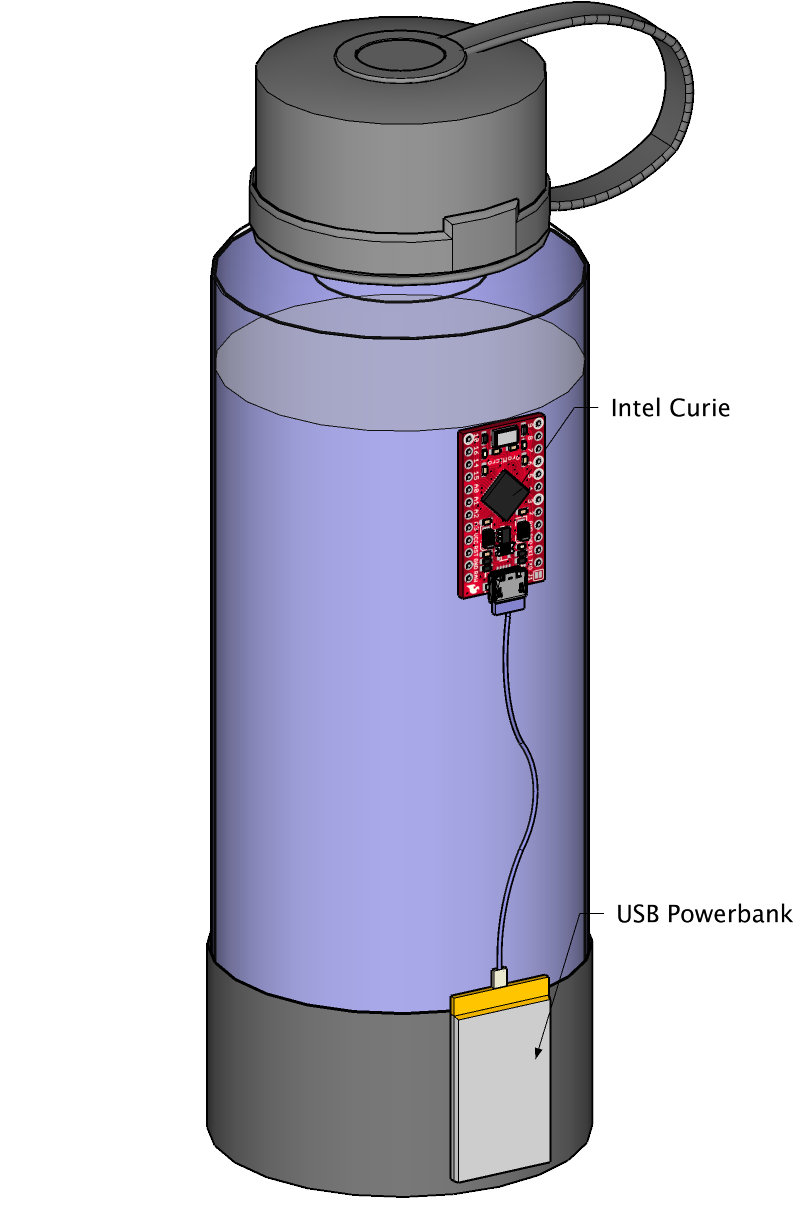
\includegraphics[width=0.3\textwidth]{assets/SmartBottle.png}
\caption{Smart Bottle}
\end{figure}